\newpage
\subsection{Diagram komponentów}
\begin{adjustwidth}{2em}{0pt}
Diagram komponentów przedstawia podział całego systemu na mniejsze podsystemy. Komponent jest to wymienny,wykonywalny fragment systemu. Zależności między komponentami są przedstawiane w postaci interfejsów tzn. jeden komponent może korzystać z funkcji jakie udostępnia inny komponent. Na rysunku \ref{fig:diagram_komponentow} przedstawiony jest diagram komponentów projektowanego systemu

\begin{figure}[H]
    \centering
    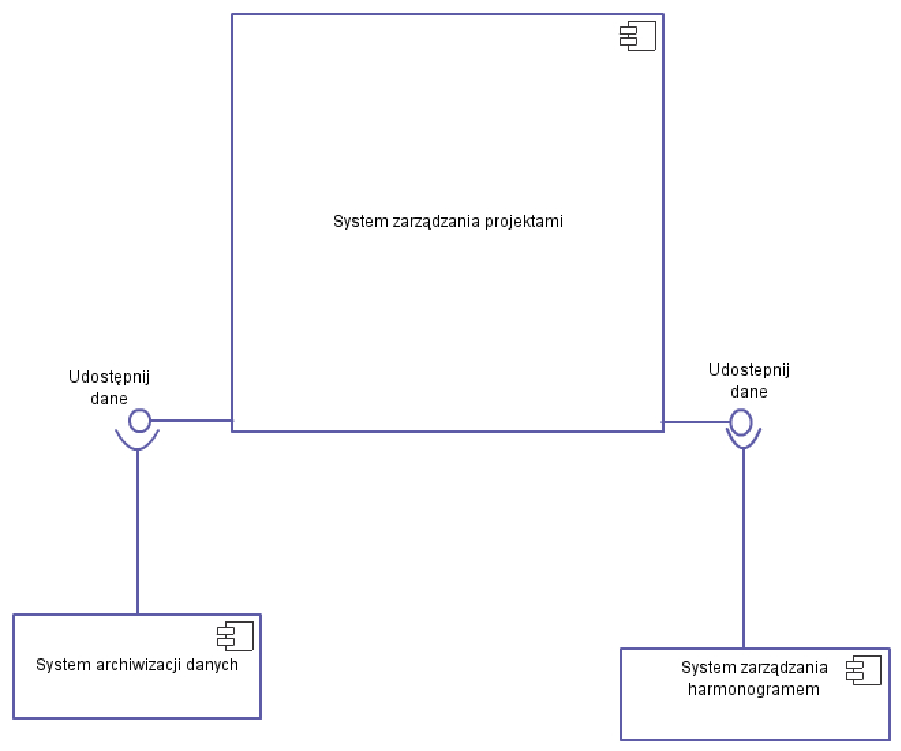
\includegraphics[scale=1]{diagramy/sekwencji_i_komponentow/diagramKomponentow.pdf}
    \caption{Diagram komponentów}
    \label{fig:diagramKomponentow.pdf}
\end{figure} 

\end{adjustwidth}
\newpage